\documentclass{report}

%%%%%%%%%%%%%%%%%%%%%%%%%% Загальна інформація %%%%%%%%%%%%%%%%%%%%%%%%%%
\Subject {Системи штучного інтелекту}
\LabTitle{Мініпакетний стохастичний градієнтний спуск}
\LabReport{Семінар}


%----------------------------------------------------
%	  Персональна інформація виконавця завдання
%----------------------------------------------------
\Done{Виконав:}  % Поставте правильне закінчення


\Surname{Стародубець}  % Вкажіть своє прізвище
\Name{Ілля}			% та ім'я
\Group {ІМ-32мп}     % група в якій навчаєтесь
\YearOfStudying {1} % курс навчання


%%%%%%%%%%%%%%%%%%%%%%%%%%	 ПОЧАТОК ЗВІТУ	 %%%%%%%%%%%%%%%%%%%%%%%%
\startDocument


\section{Вступ}
\subsection{Градієнтний спуск}

Градієнтний спуск є фундаментальним алгоритмом в області оптимізації та машинного навчання. Його основна мета полягає в пошуку мінімуму (або максимуму) функції шляхом ітеративного оновлення параметрів моделі в напрямку, протилежному градієнту цієї функції в поточній точці параметрів. Це дозволяє систематично зменшувати значення функції та знаходити оптимальні параметри.

Градієнт спуску може бути використаний для навчання моделей машинного навчання, де функція втрати визначає рівень помилок моделі. Основний алгоритм градієнтного спуску виглядає наступним чином:

Ініціалізація параметрів: Початкові значення параметрів моделі вибираються випадковим чином або за допомогою певної стратегії.

Обчислення градієнта: Обчислюється градієнт функції втрати в поточних значеннях параметрів за наступною формулою:

\[
\theta_i = \theta_i - \alpha \frac{1}{m} \sum_{j=1}^{m} (h_\theta(x^{(j)}) - y^{(j)}) \cdot x^{(j)}_i
\]

Де: 
$\theta_i$ - $i$-й параметр моделі;
$\alpha$ - швидкість навчання;
$m$ - кількість екземплярів в наборі даних;
$h_\theta(x^{(j)})$ - передбачене значення для $j$-го екземпляру;
$y^{(j)}$ - фактичне цільове значення для $j$-го екземпляру;
$x^{(j)}_i$ - $i$-й ознака $j$-го екземпляру.

Оновлення параметрів: Параметри моделі оновлюються в напрямку, протилежному градієнту, з врахуванням кроку навчання (learning rate).

Повторення: Кроки 2-3 повторюються до досягнення збіжності або визначеного числа ітерацій.

Градієнтний спуск може викликати проблеми при оптимізації великих наборів даних або функцій з великою кількістю параметрів, оскільки вимагає обчислення градієнта за всіма даними. Це призводить до значних обчислювальних витрат та може бути неефективним у випадках великих обсягів даних.

\subsection{Стохастичний градієнтний спуск}

Стохастичний градієнтний спуск (SGD) є вдосконаленою версією класичного градієнтного спуску, яка стала особливо популярною в області машинного навчання через здатність ефективно працювати з великими обсягами даних. Основна ідея полягає в тому, щоб використовувати лише частковий (випадковий) піднабір даних для оновлення параметрів моделі на кожній ітерації, замість використання усіх даних, як у класичному градієнтному спуску.

Ініціалізація параметрів: Початкові значення параметрів моделі встановлюються випадковим чином або за допомогою певної стратегії.

Епоха (ітерація): Для кожного піднабору даних (мініпакета) випадковим чином обирається підмножина даних.

Обчислення градієнта: Градієнт функції втрати обчислюється лише для вибраного мініпакету за наступною формулою:

\[
\theta_i = \theta_i - \alpha (h_\theta(x^{(j)}) - y^{(j)}) \cdot x^{(j)}_i
\]

Де:
$\theta_i$ - $i$-й параметр моделі;
$\alpha$ - швидкість навчання;
$h_\theta(x^{(j)})$ - передбачене значення для $j$-го екземпляру;
$y^{(j)}$ - фактичне цільове значення для $j$-го екземпляру;
$x^{(j)}_i$ - $i$-й ознака $j$-го екземпляру.

Оновлення параметрів: Параметри моделі оновлюються в напрямку, протилежному градієнту, застосованому до обраного мініпакету.

Повторення: Кроки 2-4 повторюються для кожного мініпакету та до досягнення збіжності або визначеного числа ітерацій.

Стохастичний градієнтний спуск відмінний від градієнтного спуску тим, що його оновлення параметрів є більш частковим та швидким, що робить його ефективнішим для великих наборів даних. Однак він також може призводити до менш стабільної збіжності, оскільки кожне оновлення базується лише на обмеженому піднаборі даних.

Для вирішення цього, інші модифікації SGD, такі як мініпакетний стохастичний градієнтний спуск (Mini-batch SGD), розглядають використання невеликого, але не повністю випадкового, піднабору даних, що дозволяє підтримувати баланс між обчислювальною ефективністю та стабільністю збіжності.

\subsection{Роль мініпакетного підходу у великих наборах даних}

Зі збільшенням обсягу даних у сучасних завданнях машинного навчання виникає проблема ефективності обчислень при застосуванні класичних оптимізаційних методів, зокрема градієнтного спуску. Мініпакетний підхід вирішує цю проблему: при навчанні моделі градієнти параметрів оцінюються на піднаборі даних (мініпакетів), що вибирається випадковим чином зі всього набору даних, що в свою чергу дозволяє ефективно працювати з великими обсягами даних. Розглянемо роль мініпакетного підходу у великих наборах даних.

Ефективність обчислень: великі набори даних можуть суттєво ускладнити обчислювальний процес. Використання мініпакетів дозволяє обробляти лише обмежену кількість даних на кожній ітерації, що суттєво зменшує вимоги до ресурсів.

Адаптація до обмежень пам'яті: Великі обсяги даних можуть вимагати значних обсягів пам'яті для зберігання та обробки. Використання мініпакетів дозволяє працювати з частковими наборами даних, що полегшує управління обмеженнями пам'яті.

Збереження стохастичності: використання випадково вибраних мініпакетів допомагає зберегти стохастичність у процесі навчання. Це може бути корисним для уникнення застрягання в локальних мінімумах та покращення загальної збіжності моделі.

Підвищення загальної збіжності: мініпакетний підхід може сприяти швидшій збіжності моделі, оскільки оновлення параметрів проводяться частіше, а отже, модель може швидше адаптуватися до нових даних.

Можливість паралельності: обробка мініпакетів може бути паралельною, що дозволяє використовувати високопродуктивне обладнання та багатоядерні обчислювальні ресурси для прискорення процесу.





\section{Мініпакетний стохастичний градієнтний спуск}

\subsection{Основні принципи та визначення}

Мініпакетний стохастичний градієнтний спуск (Mini-batch Stochastic Gradient Descent, Mini-batch SGD) представляє собою комбінацію ідей з стохастичного градієнтного спуску та мініпакетного підходу. Він використовує випадково вибрані мініпакети даних для оновлення параметрів моделі, забезпечуючи ефективність та стабільність навчання\cite{towardsdatasciencembgd}.

\begin{figure}[H]
  \center
  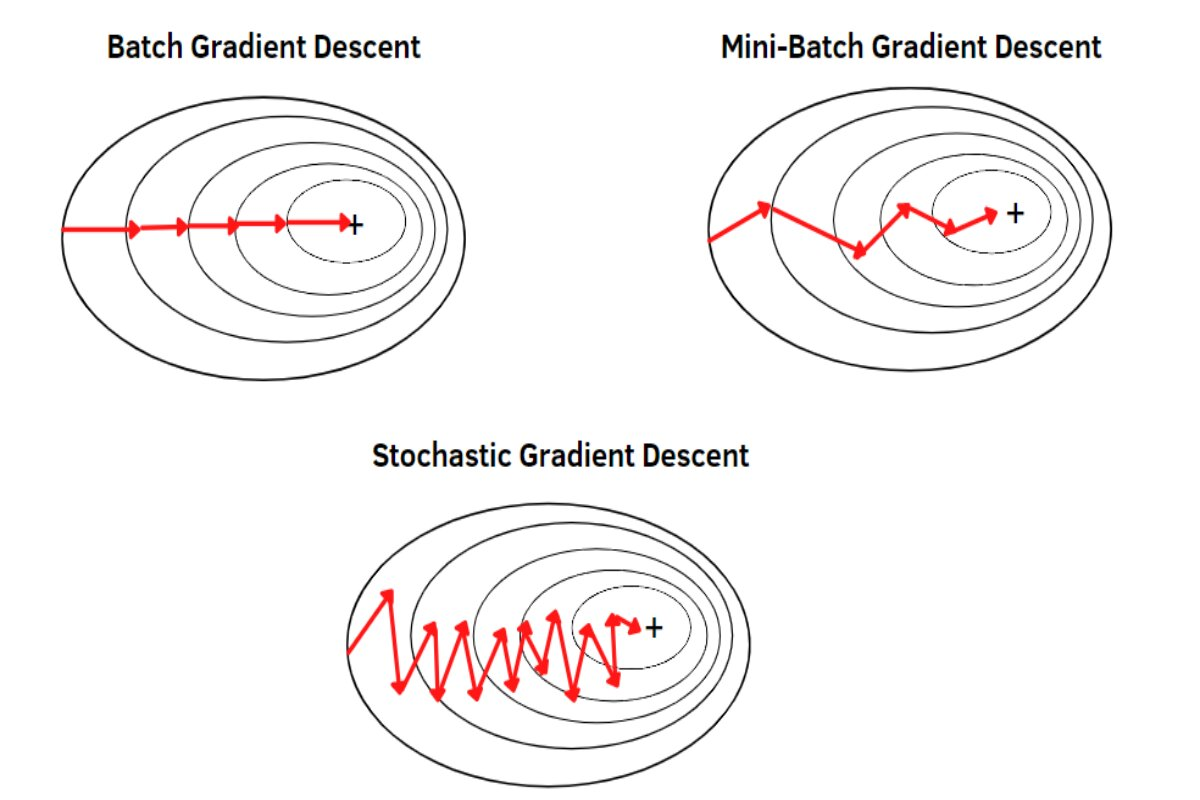
\includegraphics[width=0.8\textwidth]{gradient_descent}
  \caption{Наближення до мінімуму у різних варіаціях градієнтного спуску \cite{statusneombgd}}
  \label{im:gradient_descent}
\end{figure}

Розглянемо основні принципи та визначення цього методу:

Ініціалізація параметрів: Початкові значення параметрів моделі встановлюються випадковим чином або за допомогою певної стратегії, як у стандартному градієнтному спуску.

Мініпакети даних: Набір даних розділяється на невеликі піднабори (мініпакети), кожен з яких містить обмежену кількість зразків. Такі мініпакети випадковим чином вибираються для кожної ітерації навчання.

Обчислення градієнта: Градієнт функції втрати обчислюється на основі обраного мініпакету даних, а не на всьому наборі даних, використовуючи наступну формулу:

\[
\theta_i = \theta_i - \alpha \frac{1}{B} \sum_{j \text{ в міні-батчі}} (h_\theta(x^{(j)}) - y^{(j)}) \cdot x^{(j)}_i
\]

Де: 
$\theta_i$ - $i$-й параметр моделі;
$\alpha$ - швидкість навчання;
$B$ - розмір міні-батчу;
$h_\theta(x^{(j)})$ - передбачене значення для $j$-го екземпляру;
$y^{(j)}$ - фактичне цільове значення для $j$-го екземпляру;
$x^{(j)}_i$ - $i$-й ознака $j$-го екземпляру.

Оновлення параметрів: Параметри моделі оновлюються в напрямку, протилежному градієнту, застосованому до обраного мініпакету. Цей крок повторюється для кожного нового мініпакету.

Параметри адаптації: Мініпакетний SGD може використовувати методи адаптації кроку навчання, такі як Adam або RMSprop, для автоматичного адаптування кроку навчання на основі історії градієнтів.

Повторення: Процес обчислення градієнта та оновлення параметрів повторюється для кожного нового мініпакету та до досягнення збіжності або визначеної кількості ітерацій.

Основні переваги мініпакетного стохастичного градієнтного спуску включають підвищену ефективність обчислень, здатність адаптуватися до великих наборів даних та стабільність збіжності. Використання мініпакетів дозволяє зберегти частину стохастичності, що може бути корисним для уникнення застрягання в локальних мінімумах та покращення загальної якості моделі.



\subsection{Взаємодія стохастичності та мініпакетів}

Взаємодія стохастичності та мініпакетів є ключовою особливістю методу мініпакетного стохастичного градієнтного спуску (Mini-batch SGD). Ця взаємодія визначає ефективність та динаміку процесу оптимізації в контексті навчання моделей машинного навчання.

Стабільність збіжності. Стохастичність (випадковий вибір зразків) дозволяє уникнути застрягання в локальних мінімумах та може допомагати моделі знаходити більш загальні закономірності в данних.
Мініпакети забезпечують більш стабільну траєкторію спуску, оскільки обчислення градієнта базуються на кількох зразках, а не на одному. Це допомагає зменшити випадкові коливання градієнту.
Баланс між обчислювальною ефективністю та точністю\cite{mediummbgd}:

Стохастичність дозволяє обробляти лише частину даних на кожній ітерації, зменшуючи обчислювальні витрати.
Мініпакети виступають як компроміс між повною стохастичністю (коли використовується лише один зразок) та повною детермінованістю (коли використовується весь набір даних).

Збереження стохастичності. Випадковий вибір мініпакетів допомагає зберегти стохастичність у процесі навчання, що може бути корисним для уникнення локальних мінімумів та покращення загальної збіжності.
Стабільність мініпакетів також дозволяє уникнути занадто значних коливань у градієнті, що може виникати при використанні лише одного зразка (повна стохастичність).
Зменшення дисперсії градієнта:

Мініпакети допомагають зменшити дисперсію градієнта, оскільки вони представляють собою усереднені значення градієнтів для обраного піднабору даних. Це забезпечує більш стабільний та надійний градієнт для кожного оновлення параметрів.
Взаємодія стохастичності та мініпакетів дозволяє мінімізувати обчислювальні витрати та одночасно забезпечувати стабільність та швидкість збіжності моделі. Цей підхід стає особливо важливим у великих наборах даних, де повний градієнтний спуск може бути вкрай обчислювально витратним.



\subsection{Переваги та недоліки}

Оскільки цей алгоритм комбінує мініпакетний підхід та стохастичність, його можливо вважати змішаним методом, об'єднуючи в собі як певні переваги, так і недоліки. Розглянемо в контексті порівняння його з повним градієнтним спуском.

Переваги:
\begin{enumerate}
  \item Ефективність: краще проявляє у великих наборах даних, так як дозволяє використовувати переваги швидкості стохастичного градієнтного спуску, але при цьому забезпечує більш стабільні та менш зашумлені оновлення.
  \item Збереження локальних особливостей: мініпакетний підхід може допомагати уникнути застрягання в локальних мінімумах, оскільки він користується частково випадковими вибірками для оцінки градієнта.
  \item Менша вимога до пам'яті: мініпакетний метод вимагає менше пам'яті для збереження градієнтів, оскільки він працює з випадковими підмножинами даних, а не з усією вибіркою.
  \item Можливість розпаралелювання: може бути ефективно реалізований в режимі паралельності, що дозволяє прискорити процес навчання на багатоядерних або розподілених обчислювальних системах.
  \item Висока швидкість збіжності оскільки оновлення параметрів відбуваються на кожній ітерації.
  \item Підвищена стійкість до викидів: мініпакетний підхід може бути менш чутливим до окремих викидів у навчальних даних, оскільки використовуються підмножини, а не весь набір даних.
\end{enumerate}

Недоліки:
\begin{enumerate}
  \item Нестабільність оновлень: внаслідок використання випадкових мініпакетів, оновлення можуть бути нестабільними та варіюватися від ітерації до ітерації, що може призвести до менш точного збіження.
  \item Складність вибору гіперпараметрів: оптимальний вибір гіперпараметрів, таких як розмір мініпакету та швидкість навчання, може виявитися нетривіальним завданням, і не існує універсальної конфігурації, що підходить для всіх задач.
  \item Неефективність для малих розмірів вибірки: у випадку, коли розмір вибірки дуже малий, мініпакетний метод може не бути так ефективним через великий вплив випадковості.
  \item Споживання пам'яті: Якщо розмір мініпакету великий, це може призводити до великого споживання пам'яті, особливо при обробці великих об'ємів даних.
  \item Можливий ризик перенавчання: Використання мініпакетів може збільшити ризик перенавчання, особливо якщо розмір мініпакету надто малий, і модель надто чутлива до окремих прикладів.
  \item Потреба відслідковувати та адаптуватися до змін: При великій динаміці даних, особливо якщо розподіл даних змінюється, потрібно стежити за використанням мініпакетів і, можливо, адаптувати їх розмір чи інші параметри.
\end{enumerate}



\subsection{Порівняння з іншими оптимізаційними методами}

Порівняння мініпакетного стохастичного градієнтного спуску з іншими оптимізаційними методами може залежати від конкретної задачі, обсягу даних та архітектури моделі. Ось порівняння з деякими іншими оптимізаційними методами:

\begin{enumerate}

\item Adam (Adaptive Moment Estimation):

Мініпакетний стохастичний градієнтний спуск використовує адаптивний крок навчання та моментум для кожного параметра, що може поліпшити швидкість навчання та стабільність збіжності.

Adam: Забезпечує автоматичну адаптацію кроку навчання та використовує інформацію про минулі градієнти для покращення швидкості збіжності.

\item RMSprop (Root Mean Square Propagation):

Мініпакетний стохастичний градієнтний спуск: Використовує експоненційне середнє квадратів градієнтів для адаптивного кроку навчання.

RMSprop: Забезпечує автоматичне адаптивне налаштування кроку навчання, що допомагає уникнути проблем з великими та малими градієнтами.

\item Adagrad (Adaptive Gradient Algorithm):

Мініпакетний стохастичний градієнтний спуск: Адаптивно налаштовує крок навчання для кожного параметра на основі накопичення квадратів градієнтів.

Adagrad: Підтримує різні кроки навчання для різних параметрів в залежності від їх історії градієнтів.

\item Adadelta:

Мініпакетний стохастичний градієнтний спуск: Використовує співвідношення кроків навчання між оновленнями параметрів та кроками градієнтів.

Adadelta: Адаптується до змін динаміки оптимізаційного процесу без використання глобального кроку навчання.

\end{enumerate}

Вибір конкретного методу оптимізації залежить від властивостей конкретної задачі, доступних ресурсів та швидкості збіжності, яку можна досягти. Зазвичай емпіричні експерименти на конкретних завданнях можуть допомогти визначити оптимальний метод оптимізації для конкретного випадку.



\subsection{Практичні застосування}

Мініпакетний стохастичний градієнтний спуск широко використовується в практиці машинного навчання та глибокого навчання завдяки своїм ефективним властивостям. Великі обсяги даних у великих датасетах, таких як ImageNet, диктують використання мініпакетів для ефективного навчання глибоких моделей.

Класифікація та регресія: мініпакетний підхід дозволяє ефективно працювати з великими обсягами інформації, підвищуючи швидкість навчання моделі.

Обробка природних мов (Natural Language Processing, NLP): застосовується для моделей таких як рекурентні нейронні мережі (RNN) або трансформери, які потребують значних обчислювальних ресурсів.

Зображення та комп'ютерний зір: використовується для роботи з великими датасетами зображень, де обсяг даних може бути великим викликом для ефективного навчання.

Рекомендаційні системи: в цій області моделі повинні адаптуватися до швидко змінюючих смаків та поведінки користувачів.

Застосування в глибокому навчанні: мініпакетний підхід є основою для навчання глибоких архітектур, таких як конволюційні нейронні мережі (CNN) та рекурентні нейронні мережі (RNN), які здійснюють успішні застосування у різних областях.

Аналіз даних та машинне навчання в реальному часі: мініпакетний стохастичний градієнтний спуск може бути ефективним для розв'язання завдань машинного навчання в реальному часі, де швидкість навчання та оновлення моделі є критичними.

Генерація контенту: використовується в задачах генерації контенту, таких як створення зображень або текстових послідовностей, де навчання може вимагати великого обсягу даних.

Мініпакетний стохастичний градієнтний спуск поєднує у собі краще с мініпакетного підходу та стохастичного градієнтного спусту та являється корисним у великій кількості задач машинного навчання та глибокого навчання, де обчислювальні ресурси та швидкість збіжності грають критичну роль.



\section{Висновки}

Мініпакетний стохастичний градієнтний спуск широко використовується в глибокому навчанні представляє собою компроміс між обчислювальною ефективністю та стабільною збіжністю, що робить його важливим інструментом для тренування нейронних мереж на великих обсягах даних. Майбутнє Mini-batch SGD обіцяє залишатися невід'ємною ключовою складовою багатьох алгоритмів оптимізації в глибокому навчанні. Цей методта залишається ключовим інструментом у галузі машинного навчання та глибокого навчання, дозволяючи ефективно тренувати моделі на великих обсягах даних та вирішувати складні завдання та завдяки своїй ефективності та здатності пристосовуватися до різноманітних завдань, завжди матиме значущий вплив та буде певною основою для доцільного навчання на великих обсягах даних.



\newpage
%%%%%%%%%%%%%%%%%% Література %%%%%%%%%%%%%%%%%%%%%%%%%%%%%%%%%%%%%%%%%%%%%%%
\clearpage
\bibliographystyle{IEEEtran}
\bibliography{ref}
\end{document}
